\section{Aufbau des Frameworks}

\subsection{System- und Softwareumgebung}
Das Framework wurde für die Nutzung in der JupyterLab-Umgebung entwickelt, um eine plattformunabhängige und benutzerfreundliche Arbeitsumgebung zu bieten. Durch den Einsatz von Tools wie Poetry zur Verwaltung von Abhängigkeiten und Bibliotheken wie ipywidgets und pythreejs zur interaktiven 3D-Visualisierung wird eine stabile und effiziente Nutzung ermöglicht.

Abbildung~\ref{fig:verteilungsdiagramm} visualisiert das Zusammenspiel der einzelnen Softwarekomponenten innerhalb des Frameworks.
Dabei wird deutlich, wie die verschiedenen Technologien – von der Serverbereitstellung über die Paketverwaltung bis hin zur 3D-Visualisierung
und interaktiven Steuerung – ineinandergreifen, um eine stabile, plattformunabhängige und benutzerfreundliche Entwicklungsumgebung bereitzustellen.

\vspace{1em}

    \begin{figure}[H]
        \centering
        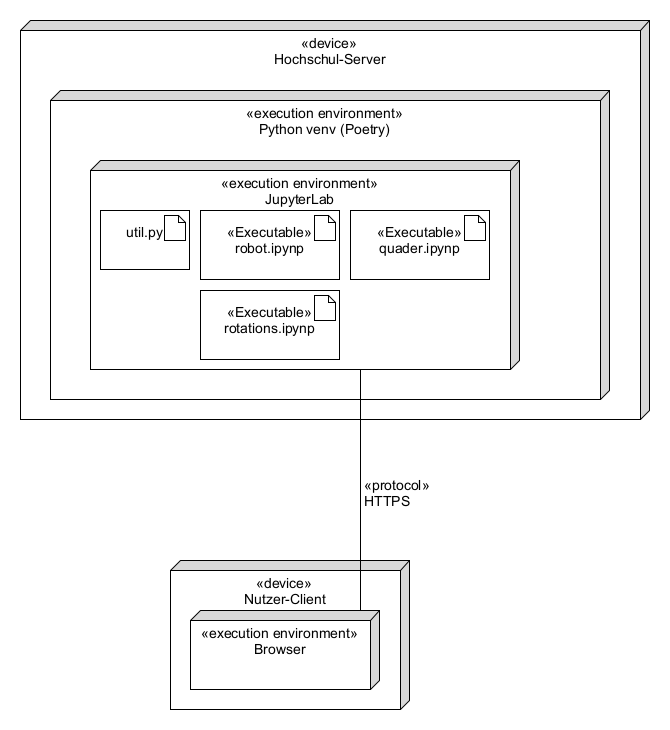
\includegraphics[width=0.9\textwidth]{images/diagramme/komponentendiagramm.png}
        \caption{Verteilungsdiagramm des Frameworks}
        \label{fig:verteilungsdiagramm}
    \end{figure}

\vspace{1em}

Das Framework ist, wie gefordert für die Nutzung innerhalb der JupyterLab-Umgebung ausgelegt.
Die Fachhochschule Dortmund stellt hierfür einen eigenen JupyterLab-Server bereit,
auf den sowohl über eine VPN-Verbindung als auch direkt im Hochschulnetz zugegriffen werden kann.
Dadurch ist keine lokale Installation erforderlich, und die Arbeitsumgebung steht einheitlich auf verschiedenen Endgeräten zur Verfügung.

Um eine einfache Einrichtung des Frameworks auf dem Server zu gewährleisten, ist es erforderlich, Versionskonflikte zwischen den verwendeten Abhängigkeiten zu vermeiden.
Zu diesem Zweck wird das Werkzeug Poetry eingesetzt.
Poetry ermöglicht die Verwaltung aller benötigten Python-Bibliotheken in festen Versionen und erstellt eine isolierte virtuelle Umgebung,
in der alle Abhängigkeiten konsistent installiert sind. Dadurch wird sichergestellt,
dass das Framework unabhängig von der Zielumgebung stabil und reproduzierbar ausgeführt werden kann.

Die Bibliothek ipywidgets wurde verwendet, um das Framework interaktiv zu gestalten.
Mithilfe von Schiebereglern, Dropdown-Menüs und Checkboxen lassen sich Rotationen der gerenderten Objekte in weicher Echtzeit anpassen.
Darüber hinaus ermöglichen die interaktiven Elemente eine benutzerfreundliche Steuerung weiterer Funktionen und tragen wesentlich zur intuitiven Bedienbarkeit des Frameworks bei.

Eine der zentralen Bibliotheken innerhalb des Projekts ist NumPy, eine weit verbreitete Python-Bibliothek für numerische Berechnungen.
NumPy wird im Kontext dieses Projekts hauptsächlich für erweiterte mathematische Operationen im Bereich der linearen Algebra eingesetzt.
Außerdem ist NumPy mit der Bibliothek SymPy, die für symbolische Mathematik verwendet wird gut kompatibel.
Diese Kompatibilität ist ebenfalls eine Anforderung im Projekt.
Obwohl NumPy eine leistungsfähige Grundlage für numerische Berechnungen bietet,
enthält es keine Funktionen für spezielle geometrische Transformationen wie die Umwandlung von Euler-Winkeln in Quaternionen oder Rotationsmatrizen – oder deren Umkehrung.
Daher wurde ergänzend die Bibliothek scipy.spatial verwendet, die solche Operationen effizient bereitstellt.


Darüber hinaus ist pythreejs als weitere wichtige Abhängigkeit integriert.
Es handelt sich hierbei um eine Python-Wrapper-Bibliothek für die JavaScript-Bibliothek three.js, die auf WebGL basiert.
pythreejs ermöglicht die Darstellung und Interaktion mit 3D-Geometrien innerhalb eines WebGL-Renderers.
Hierbei wird mithilfe von pythreejs JavaScript-Code generiert und im Hintergrund automatisch auf dem Client des Nutzers ausgeführt.
Die Visualisierung erfolgt somit lokal im Webbrowser innerhalb des Notebooks, wo auch die Steuerung über Python stattfindet.
Der Renderer kann daher nahtlos in der JupyterLab-Umgebung eingebettet und somit direkt in einem Jupyter Notebook visualisiert und gesteuert werden.
Außerdem können auf diese weise Geometrien mit Grafikbeschleunigung gerendert werden. 

Durch den Einsatz dieser Technologien wird eine effiziente und plattformunabhängige Darstellung sowie Manipulation komplexer
geometrischer Strukturen innerhalb des Frameworks ermöglicht.



\newpage


Tabelle \ref{tab:technologien} gibt einen Überblick über die zentralen Softwaretechnologien,
die für die Implementierung des Frameworks verwendet wurden. Diese Komponenten unterstützen verschiedene Aspekte wie numerische Berechnungen,
interaktive Steuerung und 3D-Visualisierung.

\vspace{1em}
    \begin{table}[H]
        \centering
        \begin{tabular}{|p{3.5cm}|p{2cm}|p{8cm}|}
        \hline
        Kategorie                   & Technologie                   & Beschreibung  \\ \hline
        Programmiersprache          & Python                        & Hochsprachige, interpretierte Programmiersprache mit Fokus auf Lesbarkeit und Einfachheit – ideal für wissenschaftliches Rechnen, Datenanalyse und Prototyping.        \\ \hline
        Laufzeitumgebung            & JupyterLab                    & Web-basierte Entwicklungsumgebung für interaktive Notebooks        \\ \hline
        Paketmanager                & Poetry                        & Verwaltung von Abhängigkeiten und virtuellen Umgebungen        \\ \hline
        Mathe-Bibliothek            & Numpy                         & Bibliothek für numerische Berechnungen und lineare Algebra        \\ \hline
        3D-Rendering                & pythreejs                     & Python-Wrapper für three.js zur Darstellung von 3D-Geometrien in Notebooks        \\ \hline
        Interaktivität              & ipywidgets                    & Erlaubt die Erstellung interaktiver GUI-Elemente wie Schieberegler, Dropdowns und Buttons in Jupyter-Notebooks        \\ \hline
        \end{tabular}
        \caption{Überblick über die im Projekt verwendeten Softwaretechnologien}
        \label{tab:technologien}
    \end{table}
\vspace{1em}

\newpage


\subsection{Framework-Library (Implementierungsdetails)}
Die Bibliothek des Frameworks besteht aus einer zentralen Datei, util.py.
In dieser Datei sind sämtliche Kernfunktionen implementiert, die zur Erstellung, Transformation und Animation geometrischer Formen benötigt werden.
Darüber hinaus enthält util.py eine Reihe von Hilfsfunktionen,
die unter anderem die Umrechnung zwischen verschiedenen Darstellungsformen von Rotationen ermöglichen sowie die Erstellung von Koordinatensystemen unterstützen.

Ergänzend dazu stellt die Bibliothek eine Klasse namens Environment bereit.
Environment repräsentiert den Renderer mit einer Szene, die eine Kamera, Beleuchtung,
ein Standardkoordinatensystem sowie ein Gitter enthält. Ein Objekt dieser Klasse kann vom Nutzer individuell angepasst werden.
So lässt sich beispielsweise festlegen, ob – abweichend vom Standard – nicht die z-Achse, sondern die y-Achse nach oben zeigt.
Auch das Gitter kann in seiner Auflösung verändert werden, indem die Größe der einzelnen Zellen angepasst wird – das Gitter kann somit feiner oder gröber dargestellt werden.

Zur Darstellung innerhalb eines Jupyter Notebooks kann ein Environment-Objekt über die dort übliche display()-Funktion gerendert werden.
Darüber hinaus besteht die Möglichkeit, interaktive Widgets für beliebige Objekte hinzuzufügen, etwa zur Steuerung der Rotation über Schieberegler.
Diese Widgets werden unterhalb des Renderers angezeigt und ermöglichen eine benutzerfreundliche Interaktion mit der Szene.

Zusätzlich enthält die Bibliothek eine Funktion move(robot, vel, steps),
mit der die Bewegung eines radgetriebenen Roboters in einer Ebene simuliert werden kann.
Die Funktion nimmt als Parameter ein Roboterobjekt, eine Geschwindigkeitsangabe sowie die Anzahl der Zeitschritte entgegen und berechnet daraus die neue Position des Roboters im Raum.

\subsection{Beispiel-Notebooks}
Das Framework enthält drei Beispiel-Notebooks, die die Anwendungsmöglichkeiten und Funktionalität praxisnah demonstrieren.
Sie sollen dem Aufgabensteller als Orientierung dienen um mithilfe des Frameworks Aufgaben oder Umgebungen zum Lernen zu generieren.

\subsubsection{robot.ipynb}
Eines dieser Notebooks trägt den Namen robot.ipynb und dient der Veranschaulichung einer einfachen Steuerungsaufgabe.
In diesem Notebook wird ein dreidimensional visualisierter Roboter mit Differentialantrieb dargestellt.
Zusätzlich wird ein vorgegebener Pfad angezeigt, den der Roboter abfahren soll. Die Aufgabe besteht darin,
die entsprechenden Antriebsgeschwindigkeiten zu berechnen und anschließend die Funktion move(robot, vel, steps) mit diesen Werten aufzurufen.
Das Notebook Orientiert sich an einer Übungsaufgabe der Fachhochschule Dortmund im Modul Robotik aus dem Jahr 2024

\begin{quote}
    \textit{Gegeben ist ein mobiler Roboter mit Differentialantrieb, der den im Weltkoordinatensystem abgebildeten Kurs von $A$ nach $C$ vorwärts abfährt.
    Der Kurs besteht aus einem Halbkreis zwischen den Punkten $A=(4,9)$ und $B=(11,2)$ und zwischen $B$ und $C=(18,9)$ aus einer Geraden. Die Positionen der Punkte sind in $m$ angegeben.}

    \vspace{1em}

        \begin{center}[H]
        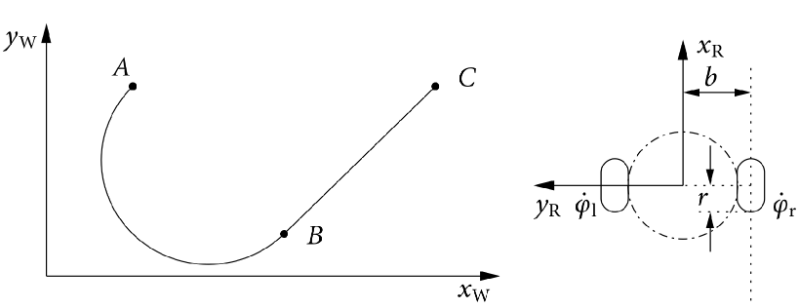
\includegraphics[width=1.0\textwidth]{images/uebung_robot.PNG}
        \end{center}

    \vspace{1em}

    \textit{Der Roboter soll den gesamten Kurs mit einer konstanten Lineargeschwindigkeit von $\dot{x_R}=1\frac{m}{s}$ abfahren.
    Beschleunigungs- und Verzögerungsvorgänge sollen vernachlässigt werden. Der Roboter hat einen halben Radabstand von $b=0.5m$ und Radradius von $0,25m$.}

    \textit{[...]}

    \textit{Welche Geschwindigkeiten in Roboterkoordinaten $(v_R=\dot{x_R}=(\dot{x_R},dot{y_R},\dot{\theta})^T)$ ergeben sich für die beiden Abschnitte jeweils? [...]}

    

\end{quote}


Nach Ausführung der jeweiligen Zelle beginnt der Roboter mit der Bewegung.
Die Nutzerin bzw. der Nutzer kann dabei direkt im Jupyter Notebook beobachten, ob der Roboter dem gewünschten Pfad korrekt folgt.

\vspace{1em}

    \begin{figure}[H]
        \centering
        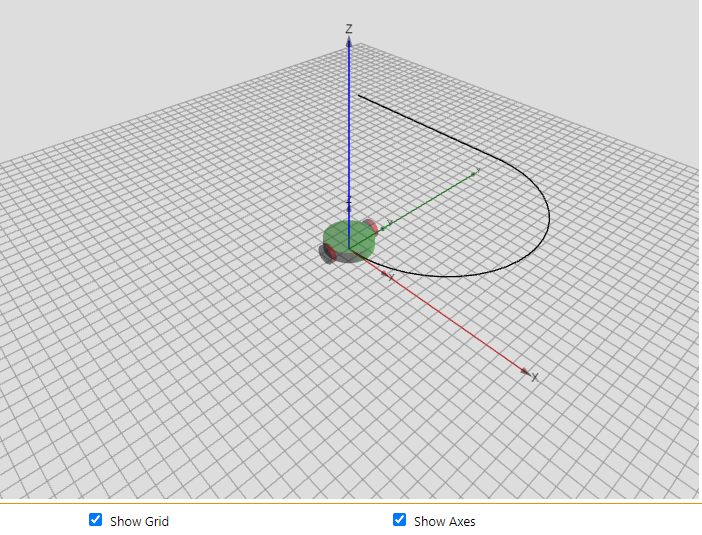
\includegraphics[width=1.0\textwidth]{images/robot.PNG}
        \caption{Verteilungsdiagramm des Frameworks (robot.ipynb während der Ausführung)}
        \label{fig:Roboter mit Differentialantrieb}
    \end{figure}

\vspace{1em}








\subsubsection{rotations.ipynb}
Ein weiteres Beispiel-Notebook trägt den Namen rotations.ipynb.
In diesem Notebook wird ein dreidimensionaler Würfel visualisiert, der vom Nutzer interaktiv transformiert werden kann.

Über integrierte Schieberegler lassen sich Translation, Rotation und Skalierung des Würfels in Echtzeit anpassen.
Ziel dieses Notebooks ist es, die Möglichkeiten des Frameworks zur Darstellung und Simulation geometrischer Transformationen zu veranschaulichen.

Die direkte visuelle Rückmeldung innerhalb des Jupyter Notebooks ermöglicht es dem Lernenden,
die Auswirkungen der jeweiligen Transformationen unmittelbar nachzuvollziehen und ein besseres Verständnis für deren Wirkung im dreidimensionalen Raum zu entwickeln.


\vspace{1em}

    \begin{figure}[H]
        \centering
        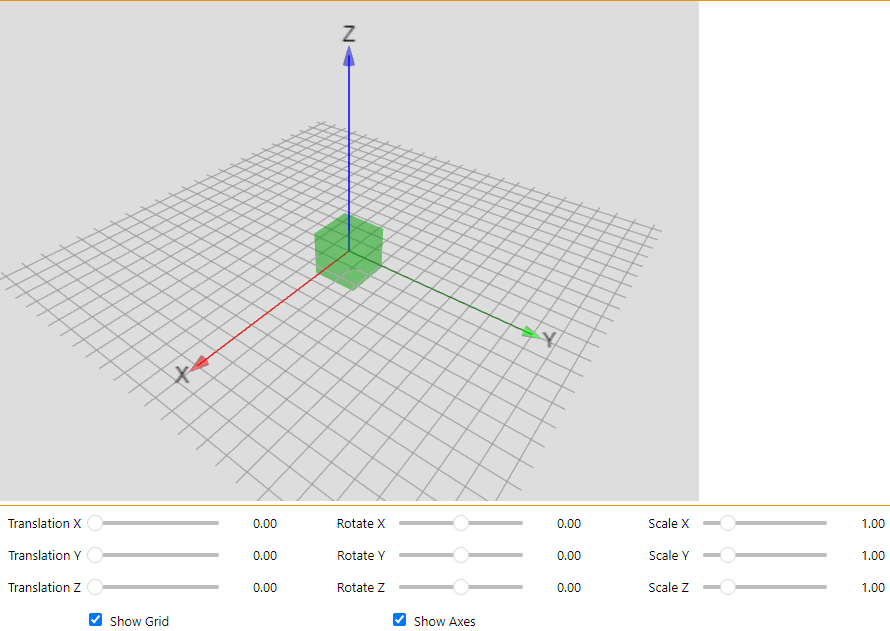
\includegraphics[width=1.0\textwidth]{images/rotations.PNG}
        \caption{Würfel mit Schiebereglern für die Rotation (rotation.ipynb während der Ausführung)}
        \label{fig:Würfel mit Schiebereglern für die Rotation}
    \end{figure}

\vspace{1em}



\subsubsection{quader.ipynb}
das andere Beispiel-Notebook trägt den Namen quader.ipynb.
Es Orientiert sich an einer Klausuraufgabe der Fachhochschule Dortmund im Modul Robotik aus dem Jahr 2010,
in der ein Quader um die Achsen des Basis-Koordinatensystems rotiert,
die jeweiligen Rotationsmatrizen aufgestellt und zu einer Gesamtrotationsmatrix zusammengefasst werden sollen.

\begin{quote}
    \textit{Gegeben ist ein quaderförmiger Körper mit den Kantenlängen $l_x=3, l_y=4$ und $l_z=2$. Eine
    Quaderecke befindet sich, wie in der nachfolgenden Abbildung dargestellt, im Ursprung eines
    ortsfesten Koordinatensystems $B$. In der Quaderecke $K$ ist ein körperfestes Koordinatensystem $K$ angebracht.}

    \vspace{1em}

        \begin{center}[H]
        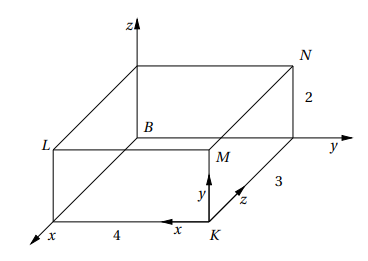
\includegraphics[width=0.6\textwidth]{images/klausur_quader.PNG}
        \end{center}

    \vspace{1em}

    \textit{Der Körper wird nun zunächst um den Winkel $\phi_z=60^\circ$ um die z-Achse, dann um den Winkel $\phi_x=-180^\circ$ um die x-Achse und schließlich um den Winkel
    $\phi_y=-90^\circ$ um die y-Achse des ortsfesten Koordinatensystems $B$ gedreht.}\par
    

    \textit{a) Stellen Sie die Rotationsmatrizen $R_x:=R(x,-180^\circ), R_y:=R(y,-90^\circ)$ und $R_z:=R(z,60^\circ)$ auf.}

    \textit{b) Berechnen Sie die Rotationsmatrix $R_G$ für die Gesamtrotation.}

    \textit{c) Welche Positinen nehmen nach der Drehung des Körpers die Körperecken $M$ und $N$ in Bezug auf das Koordinatensystem $B$ ein?}

    \textit{d) Welche Orientierung, ausgedrückt als Rotationsmatrix, hat das Koordinatensystem $K$ vor der Drehung der Körpers bezüglich der Koordinatensystems $B$?}

    \textit{e) Berechnen Sie die Eulerschen Winkel der Rotationsmatrix vor der Drehung.}

    \textit{f) Welche Orientierung, ausgedrückt als Rotationsmatrix, hat das Koordinatensystem $K$
    nach der Drehung des Körpers bezüglich des Koordinatensystems $B$?}

    \textit{g) Berechnen Sie die Roll-Nick-Gier-Winkel der Rotationsmatrix von $K$ nach der Drehung.}
\end{quote}

Das Notebook dient der Visuellen Simulation der Rotationen.
Mit der Funktion rotate\_global\_animated(mesh, angles, order) wird der Quader zunächst wie in der Aufgabe beschrieben
um die Achsen des Koordinatensystems $B$ Rotiert. Diese Transformation wird Visuell dargestellt um ein gefühl für die Rotation zu vermitteln und die Endposition aufzuzeigen.
Anschließend werden die Matrizen als Variablen aufgestellt, zusammengefasst und an die Funktion apply\_rot\_matrix\_animated(mesh, rot\_mat, speed, show\_rot\_mat) übergeben, sodass
die Rotation des Quaders anhand der Rotationsmatrix betrachtet und mit der vorrangegangegen Transformation vergleichen werden kann. Dieses Notebook kann vom Aufgabensteller so modifiziert werden,
dass die Matrizen von den Lernenden ausgefüllt werden müssen.



\vspace{1em}

    \begin{figure}[H]
        \centering
        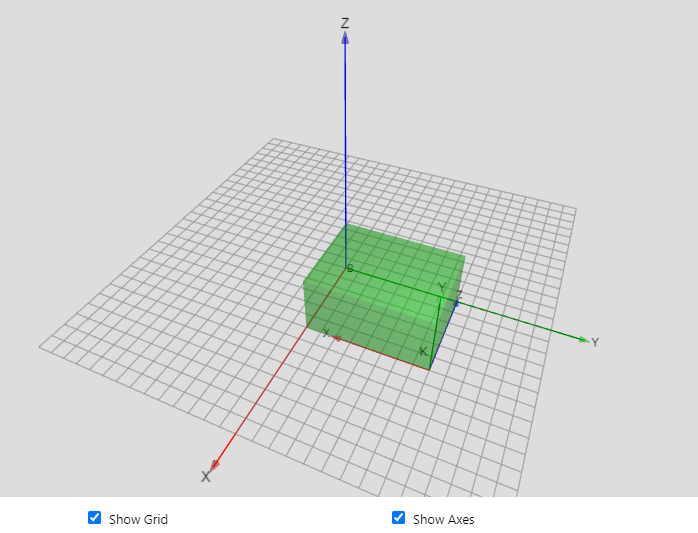
\includegraphics[width=1.0\textwidth]{images/quader.PNG}
        \caption{Quader aus der Klausuraufgabe (robot.ipynb während der Ausführung)}
        \label{fig:Quader aus der Klausuraufgabe}
    \end{figure}

\vspace{1em}

